\documentclass{article}
\usepackage{tikz}
\usepackage{mathpazo}
\usepackage{xcolor}
\usepackage{verbatim}
\usepackage{ifthen}
\usepackage[paperwidth=6in,paperheight=5in,top=0.55in,bottom=0.5in,left=0.5in,right=0.5in]{geometry}

% kill margins
\setlength{\headheight}{0cm}
\setlength{\footskip}{0cm}

% No indentation
\setlength{\parindent}{0cm}

% no page numbers
\pagenumbering{gobble}

\newcounter{row}
\newcounter{col}

% Scaling factor for KenKen grid
\edef\puzzlescale{1.2}
\edef\numrows{4}
\edef\numargs{8}

\newcommand\setrow[\numargs]{
  \setcounter{col}{1}
  \foreach \n in {#1, #2, #3, #4} {
    \edef\x{\value{col} - 1}
    \edef\y{1 + \numrows - \value{row}}
    \node[anchor=north west,scale=0.75*\puzzlescale] at (\x, \y) {\n};
    \stepcounter{col}
  }

  \ifthenelse{\equal{\showPuzzle}{false} }{
    \setcounter{col}{1}
    \foreach \n in {#5, #6, #7, #8} {
      \edef\x{\value{col} - 1}
      \edef\y{1 + \numrows - \value{row}}
      \node[anchor=center, scale=\puzzlescale] at (\x+0.5, \y-0.5) {\n };
      \stepcounter{col}
    }
  }
  {
     % false - do nothing
  }
  \stepcounter{row}
} % \setrow

\newcommand\boldh[3]{
  \edef\y{\numrows-#1}
  \edef\x{#2}
  \edef\z{\x + #3}
  \draw[ultra thick] (\x, \y) -- (\z, \y);
} % \boldh

\newcommand\boldv[3]{
  \edef\y{\numrows-#1}
  \edef\x{#2}
  \edef\z{\y - #3}
  \draw[ultra thick] (\x, \y) -- (\x, \z);
} % \boldv

\definecolor{shadegray}{gray}{0.75}

\newcommand\shadebox[2]{
  \edef\y{\numrows-#1}
  \edef\x{#2}
  \fill[shadegray] (\x, \y) rectangle (\x+1,\y-1);
} % \shadebox

\newcommand{\puzzleAddress}[1]{
  \begin{titlepage}
  \vspace*{\fill}
  \begin{center}
  \textbf{\Huge #1}
      
  \bigskip

  \vspace{1.0in}
  
  \textit{Where are you sitting?  To find out, turn the card over and
    play our puzzle!}

  \bigskip
  
  \textit{Don't break the seal until you're ready to check your
    answer---\\or admit defeat!}
  
  \end{center}
  \vspace*{\fill}
  \end{titlepage}
} % \puzzleAddress

%% \puzzlePrologue
%% @depends \showPuzzle
\newcommand{\puzzlePrologue}{
  \ifthenelse{ \equal{\showPuzzle}{true}  } {
  Hello, friends! 
  Your table is named for one of the four Shakespeare plays listed
  below.  To find which, solve the KenKen puzzle, and the number in the
  shaded box will indicate your table.  Or, just identify which
  play includes the quoted line.  Have fun!
  }
  {
  \begin{center}             
    \large \textbf{Solution}
  \end{center}
  }
} % \puzzlePrologue

\newcommand{\puzzleQuote}{The Quote}

\newcommand{\puzzleListItems}{\item An Item}

\newcommand{\puzzleListSolution}{\item The answer, Act x, Scene y}

\newcommand{\puzzleGrid}{}

\newcommand{\thetablename}{}

\renewcommand{\puzzleGrid}{

  \shadebox{2}{2} % value = 2

  \draw [very thin] (0, 0) grid (4, 4);
  \boldh{0}{0}{4}
  \boldh{1}{1}{3}
  \boldh{2}{1}{3}
  \boldh{3}{0}{3}
  \boldh{4}{0}{4}
  \boldv{0}{0}{4}
  \boldv{0}{1}{3}
  \boldv{1}{2}{1}
  \boldv{3}{2}{1}
  \boldv{2}{3}{1}
  \boldv{0}{4}{4}

  \setcounter{row}{1}
  \setrow {$6+$} {$12\times$} {} {} {2} {1} {3} {4}
  \setrow {} {$2$} {$3-$} {} {3} {2} {4} {1}
  \setrow {} {$2\div$} {} {$6+$} {1} {4} {2} {3}
  \setrow {$1-$} {} {} {} {4} {3} {2} {1}
}

%% @depends \puzzleQuote
%% @depends \puzzleListItems
%% @depends \puzzleListSolution
%% @depends \puzzleGrid
\newcommand{\puzzleBody}{

\begin{minipage}[center]{0.60\textwidth}

  \bigskip
  
  \parbox{0.85\textwidth}{
      \raggedright
      \noindent
      \textit{\puzzleQuote}
  }

  \begin{enumerate}
  \setlength{\itemsep}{1pt}
  \ifthenelse{ \equal{\showPuzzle}{true}  }
  {
      \puzzleListItems
  }
  {
      \puzzleListSolution
  }
  \end{enumerate}
\end{minipage}
%
\begin{minipage}[center]{0.38\textwidth}
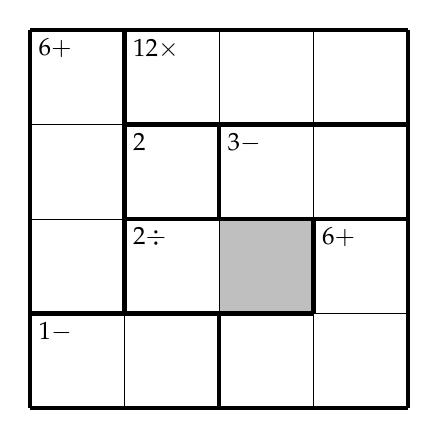
\begin{tikzpicture}[scale=\puzzlescale]

  \begin{scope}

    \puzzleGrid
    
  \end{scope}

\end{tikzpicture}
\end{minipage}
} % \puzzleBody

%% true=show puzzle, false=show solution
\newcommand{\showPuzzle}{true}

%% \puzzleEpilogue{\showPuzzle}
%% @depends \thetablename
%% @depends \showPuzzle
\newcommand{\puzzleEpilogue}{
  \ifthenelse{ \equal{\showPuzzle}{true}  } 
  {
    \textbf{Rules for KenKen}: Fill in the boxes with the numbers 1 through 4, 
    with each number appearing exactly once in every row and column.  Each
    ``cage'' (set of boxes outlined in bold) has a target number
    and mathematical operation in the top-left; combining each
    number in the cage with the operation must result in the target.
    \textit{Hint}: For cages with no operation, just fill in the target number.

    \begin{center}   
      \textit{Solutions may be found on the inside of the card.}
    \end{center}
  }
  {
   \begin{center}
     \large \textit{See you at Table} \thetablename!
   \end{center}
  }
} % \puzzleEpilogue

%% @depends \showPuzzle
\newcommand{\makepuzzle}{

\puzzlePrologue

\medskip

\puzzleBody

\bigskip

\puzzleEpilogue

} % \makepuzzle

%% @depends \thetablename
\newcommand{\makePuzzleCard}[1]{

\renewcommand{\showPuzzle}{true}

\puzzleAddress{#1}

\pagebreak

\makepuzzle

\pagebreak

\renewcommand{\showPuzzle}{false}

\makepuzzle

\pagebreak

} % \makePuzzleCard


\newcommand{\setPuzzleHamlet}
{
  \renewcommand{\thetablename}{Hamlet}

  \renewcommand{\puzzleQuote}{
  ``Use every man after his desert, and who should scape whipping?  
    Use them after your own honour and dignity---the less they deserve, 
    the more merit is in your bounty.''
  }

  \renewcommand{\puzzleListItems}{
      \item Twelfth Night
      \item Hamlet
      \item Much Ado About Nothing
      \item The Taming of the Shrew
  } % \puzzleListItems

  \renewcommand{\puzzleListSolution}{
      \setcounter{enumi}{1}
      \item \textbf{Hamlet}, Act~2, Scene~2
  } % \puzzleListSolution

} % \setPuzzleHamlet

\newcommand{\setPuzzleMuchAdo}
{
  \renewcommand{\thetablename}{Much Ado About Nothing}

  \renewcommand{\puzzleQuote}{
  ``Shall quips and sentences and these paper bullets of the brain awe a man 
    from the career of his humour? No. The world must be peopled. 
    When I said I would die a bachelor, 
    I did not think I should live till I were married.''
  }

  \renewcommand{\puzzleListItems}{
      \item Hamlet
      \item Much Ado About Nothing
      \item The Taming of the Shrew
      \item A Midsummer Night's Dream
  } % \puzzleListItems

  \renewcommand{\puzzleListSolution}{
      \setcounter{enumi}{1}
      \item \textbf{Much Ado About Nothing}, Act~2, Scene~3
  } % \puzzleListSolution

} % \setPuzzleMuchAdo

\newcommand{\setPuzzleTwelfthNight}
{
  \renewcommand{\thetablename}{Twelfth Night}

  \renewcommand{\puzzleQuote}{
  ``What means this lady?
\phantom{``}Fortune forbid my outside have not charmed her. \linebreak
\phantom{``}She made good view of me, indeed so much \linebreak
\phantom{``}That straight methought her eyes hod lost her tongue.''
  }

  \renewcommand{\puzzleListItems}{
      \item Antony and Cleopatra
      \item Twelfth Night
      \item Hamlet
      \item Much Ado About Nothing
  } % \puzzleListItems

  %% @todo
  \renewcommand{\puzzleListSolution}{
      \setcounter{enumi}{1}
      \item \textbf{Twelfth Night}, Act~2, Scene~2  } % \puzzleListSolution

} % \setPuzzleTwelfthNight

\newcommand{\setPuzzleRomeoAndJuliet}
{
  \renewcommand{\thetablename}{Romeo And Juliet}

  \renewcommand{\puzzleQuote}{
  ``If thou dost love, pronounce it faithfully; \linebreak
\phantom{``}Or if thou think'st I am too quickly won,  \linebreak
\phantom{``}I'll frown, and be perverse, and say thee nay,  \linebreak
\phantom{``}So thou wilt woo; but else, not for the world.''
  }

  \renewcommand{\puzzleListItems}{
      \item A Midsummer Night's Dream
      \item Romeo and Juliet
      \item As You Like It
      \item Antony and Cleopatra
  } % \puzzleListItems

  \renewcommand{\puzzleListSolution}{
      \setcounter{enumi}{1}
    \item \textbf{Romeo and Juliet}, Act~2, Scene~1
  } % \puzzleListSolution

} % \setPuzzleRomeoAndJuliet

\newcommand{\setPuzzleTamingOfTheShrew}
{
  \renewcommand{\thetablename}{Taming of the Shrew}

  %% @todo
  \renewcommand{\puzzleQuote}{
  ``You have showed a tender fatherly regard, \linebreak
\phantom{``}To wish me wed to one half-lunatic, \linebreak
\phantom{``}A madcap ruffian and a swearing Jack, \linebreak
\phantom{``}That thinks with oaths to face the matter out.''
  }

  \renewcommand{\puzzleListItems}{
      \item Much Ado About Nothing
      \item The Taming of the Shrew
      \item A Midsummer Night's Dream
      \item Romeo and Juliet
  } % \puzzleListItems

  \renewcommand{\puzzleListSolution}{
      \setcounter{enumi}{1}
      \item \textbf{Taming of the Shrew}, Act~2, Scene~1
  } % \puzzleListSolution

} % \setPuzzleTamingOfTheShrew

\newcommand{\setPuzzleMidsummerNights}
{
  \renewcommand{\thetablename}{Midsummer Night's Dream}

  \renewcommand{\puzzleQuote}{
  ``The iron tongue of midnight hath told twelve. \linebreak
\phantom{``}Lovers, to bed; 'tis almost fairy time. \linebreak
\phantom{``}I fear we shall outsleep the coming morn \linebreak
\phantom{``}As much as we this night have overwatched.''
  }

  \renewcommand{\puzzleListItems}{
      \item The Taming of the Shrew
      \item A Midsummer Night's Dream
      \item Romeo and Juliet
      \item As You Like It
  } % \puzzleListItems

  \renewcommand{\puzzleListSolution}{
      \raggedright
      \setcounter{enumi}{1}
      \item \textbf{A Midsummer Night's Dream}, \linebreak Act~5, Scene~1
  } % \puzzleListSolution

} % \setPuzzleMidsummerNights

\newcommand{\setPuzzleAsYouLikeIt}
{
  \renewcommand{\thetablename}{As You Like It}

  \renewcommand{\puzzleQuote}{
  ``Men are April when they woo, December when they wed.  
    Maids are May when they are maids, 
   but the sky changes when they are wives.''
  }

  \renewcommand{\puzzleListItems}{
      \item Romeo and Juliet
      \item As You Like It
      \item Antony and Cleopatra
      \item Twelfth Night
  } % \puzzleListItems

  \renewcommand{\puzzleListSolution}{
      \setcounter{enumi}{1}
      \item \textbf{As You Like It}, Act~4, Scene~1
  } % \puzzleListSolution

} % \setPuzzleAsYouLikeIt

\newcommand{\setPuzzleAntonyAndCleopatra}
{
  \renewcommand{\thetablename}{Antony and Cleopatra}

  \renewcommand{\puzzleQuote}{
``Come, Let’s have one other gaudy night. Call to me \linebreak
\phantom{``}All my sad captains. Fill our bowls once more. \linebreak
\phantom{``}Let’s mock the midnight bell.''
  }

  \renewcommand{\puzzleListItems}{
      \item As You Like It
      \item Antony and Cleopatra
      \item Twelfth Night
      \item Hamlet
  } % \puzzleListItems

  \renewcommand{\puzzleListSolution}{
      \setcounter{enumi}{1}
      \item \textbf{Antony and Cleopatra}, Act~3, Scene~13
  } % \puzzleListSolution

} % \setPuzzleAntonyAndCleopatra
